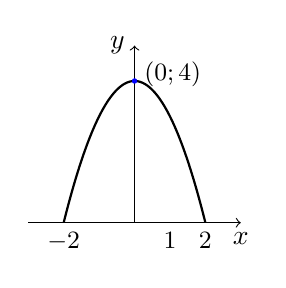
\begin{tikzpicture}[scale=0.45]
    \draw[->] (-3,0) -- (3,0) node[below] {$x$};
    \draw[->] (0,0) -- (0,5) node[left] {$y$};

    % y = 4 - x^2
    \draw[thick, domain=-2:2, samples=200] plot (\x,{4-\x*\x});

    \fill[color = blue] (0,4) circle (2.2pt);

    \node[right] at (0,4.2) {\small $(0;4)$};
    \node[below] at (-2,0) {\small $-2$};
    \node[below] at (2,0) {\small $2$};
    \node[below] at (1,0) {\small $1$};
\end{tikzpicture}
